\documentclass{article}   

\usepackage{amssymb}
\usepackage{amsfonts}
\usepackage{hyperref}
\usepackage{eqnarray,amsmath}
\usepackage[table]{xcolor}

\usepackage{listings}
\usepackage{graphicx}
\usepackage{dirtytalk}

\usepackage[table]{xcolor}
\usepackage{rotating}
\usepackage{caption}

%% if you use PostScript figures in your article
%% use the graphics package for simple commands
\usepackage{graphics}


%% or use the graphicx package for more complicated commands
\usepackage{graphicx}
\usepackage[table]{xcolor}

\usepackage[utf8]{inputenc}
 
\usepackage{listings}
\usepackage{xcolor}
 
\definecolor{codegreen}{rgb}{0,0.6,0}
\definecolor{codegray}{rgb}{0.5,0.5,0.5}
\definecolor{codepurple}{rgb}{0.58,0,0.82}
\definecolor{backcolour}{rgb}{0.95,0.95,0.92}
 
\lstdefinestyle{mystyle}{
    backgroundcolor=\color{backcolour},   
    commentstyle=\color{codegreen},
    keywordstyle=\color{magenta},
    numberstyle=\tiny\color{codegray},
    stringstyle=\color{codepurple},
    basicstyle=\ttfamily\footnotesize,
    breakatwhitespace=false,         
    breaklines=true,                 
    captionpos=b,                    
    keepspaces=true,                 
    numbers=left,                    
    numbersep=5pt,                  
    showspaces=false,                
    showstringspaces=false,
    showtabs=false,                  
    tabsize=2
}
 
\lstset{style=mystyle}
% please place your own definitions here and don't use \def but
% \newcommand{}{}
%
% Insert the name of "your journal" with
% \journalname{myjournal}
%



\begin{document}

\title{%
  Practice 1 - Basic concepts of probability. \\~\\
  \Large Environment statistics}
\author{Mayra Cristina Berrones Reyes}

\maketitle


\section{Data description}
The data used for this work comes from a government page called INEGI \cite{ine1} that according to their web site is an \say{autonomous public body responsible for regulating and coordinating the National System of Statistical and Geographical Information, as well as for capturing and disseminating information on Mexico regarding the territory, resources, population and economy, which allows to publicize the characteristics of our country and help decision making} \cite{ine1}. Here we selected the subject of environmental data to draw some important information with basic concepts of probability.\\

Among all of the subjects inside the environmental material, we decided to work with the topic of water\cite{ine3}, and see how it is used across all 32 federative states encompassed in Mexico.\\

We took the tables in \say{Origen y Destino}\cite{ine3} to review how the water resources in Mexico are distributed. The name of the columns in the file of destination where displayed as shown in Table \ref{table1}.\\

Name of the federative state contains the name of the 32 states in Mexico. Here we only had to use a small shortcut in the Sublime Text app to add the quotation marks to each name. Total, Domestic, Comercial, Industrial, Public service and Pipe are numbers that represent the volume of thousands of cubic meters. \\

\begin{center}\label{table1}
\begin{tabular}{| c | c | c | c | c | c | c |}

\hline
Name of the  & Total & Domestic & Comercial & Industrial & Public & Pipe\\  
federative  &  	&  		&			&		& services&\\  
 state  &  	&  		&			&		& &\\  
 \hline
\end{tabular}
\end{center}

\section{Working with the data}

For the propose of this practice we used the programing language of R, version 3.4.2. First we took all the columns in the document and turned them in 7 different variable names. Using the variables of \textit{Total, Domestic, Comercial, Industrial, Public services} and \textit{Pipe} we constructed a box plot to show how the numbers are distributed in all of this variables from all 32 federative states. Figure \ref{fig1} we can see the box plot of all the columns.\\

\begin{figure}[htp]
	\centering
	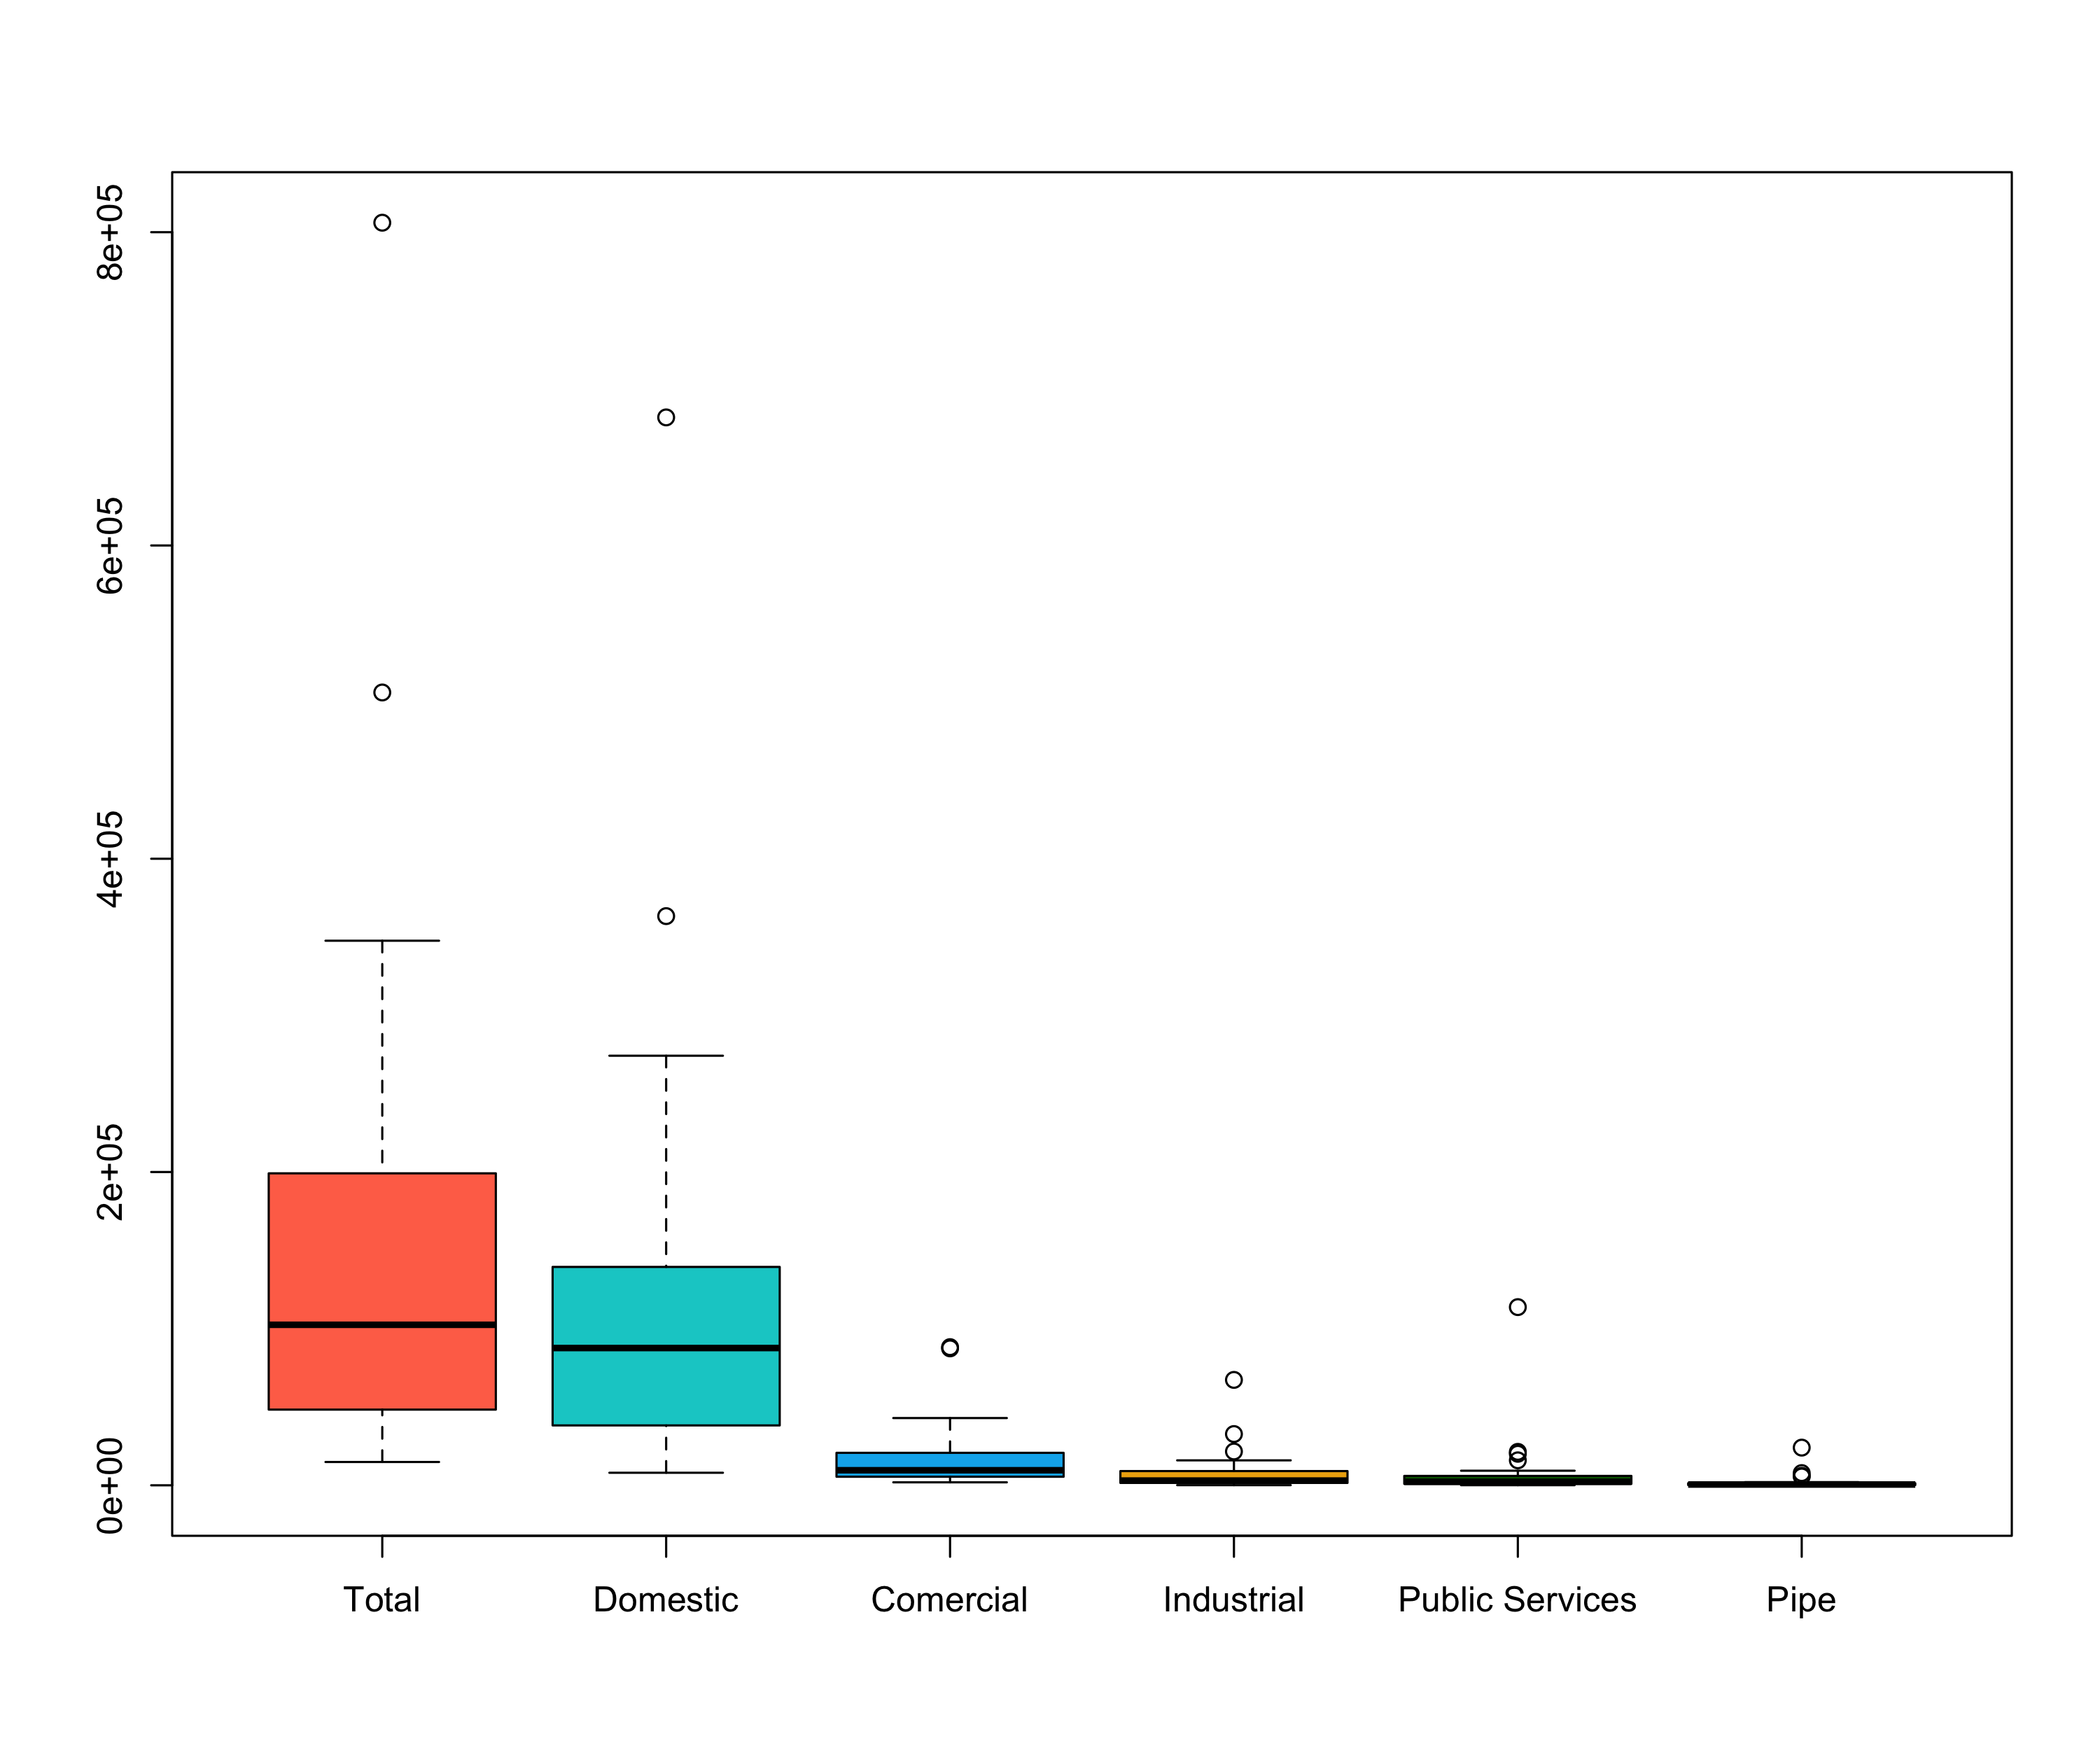
\includegraphics[width=\linewidth]{t1.png}
	\caption{Box plot of all the variables.}\label{fig1}
\end{figure}

\clearpage
 
Because the \textit{Total} and \textit{Domestic} values are significantly bigger than the other variables, the rest are barely visible. To fix this, and be able to appreciate better all the variables and outliers, in Figure \ref{fig2} we change the way we display each box plot, giving each one its individual box.\\

\begin{figure}[htp]
	\centering
	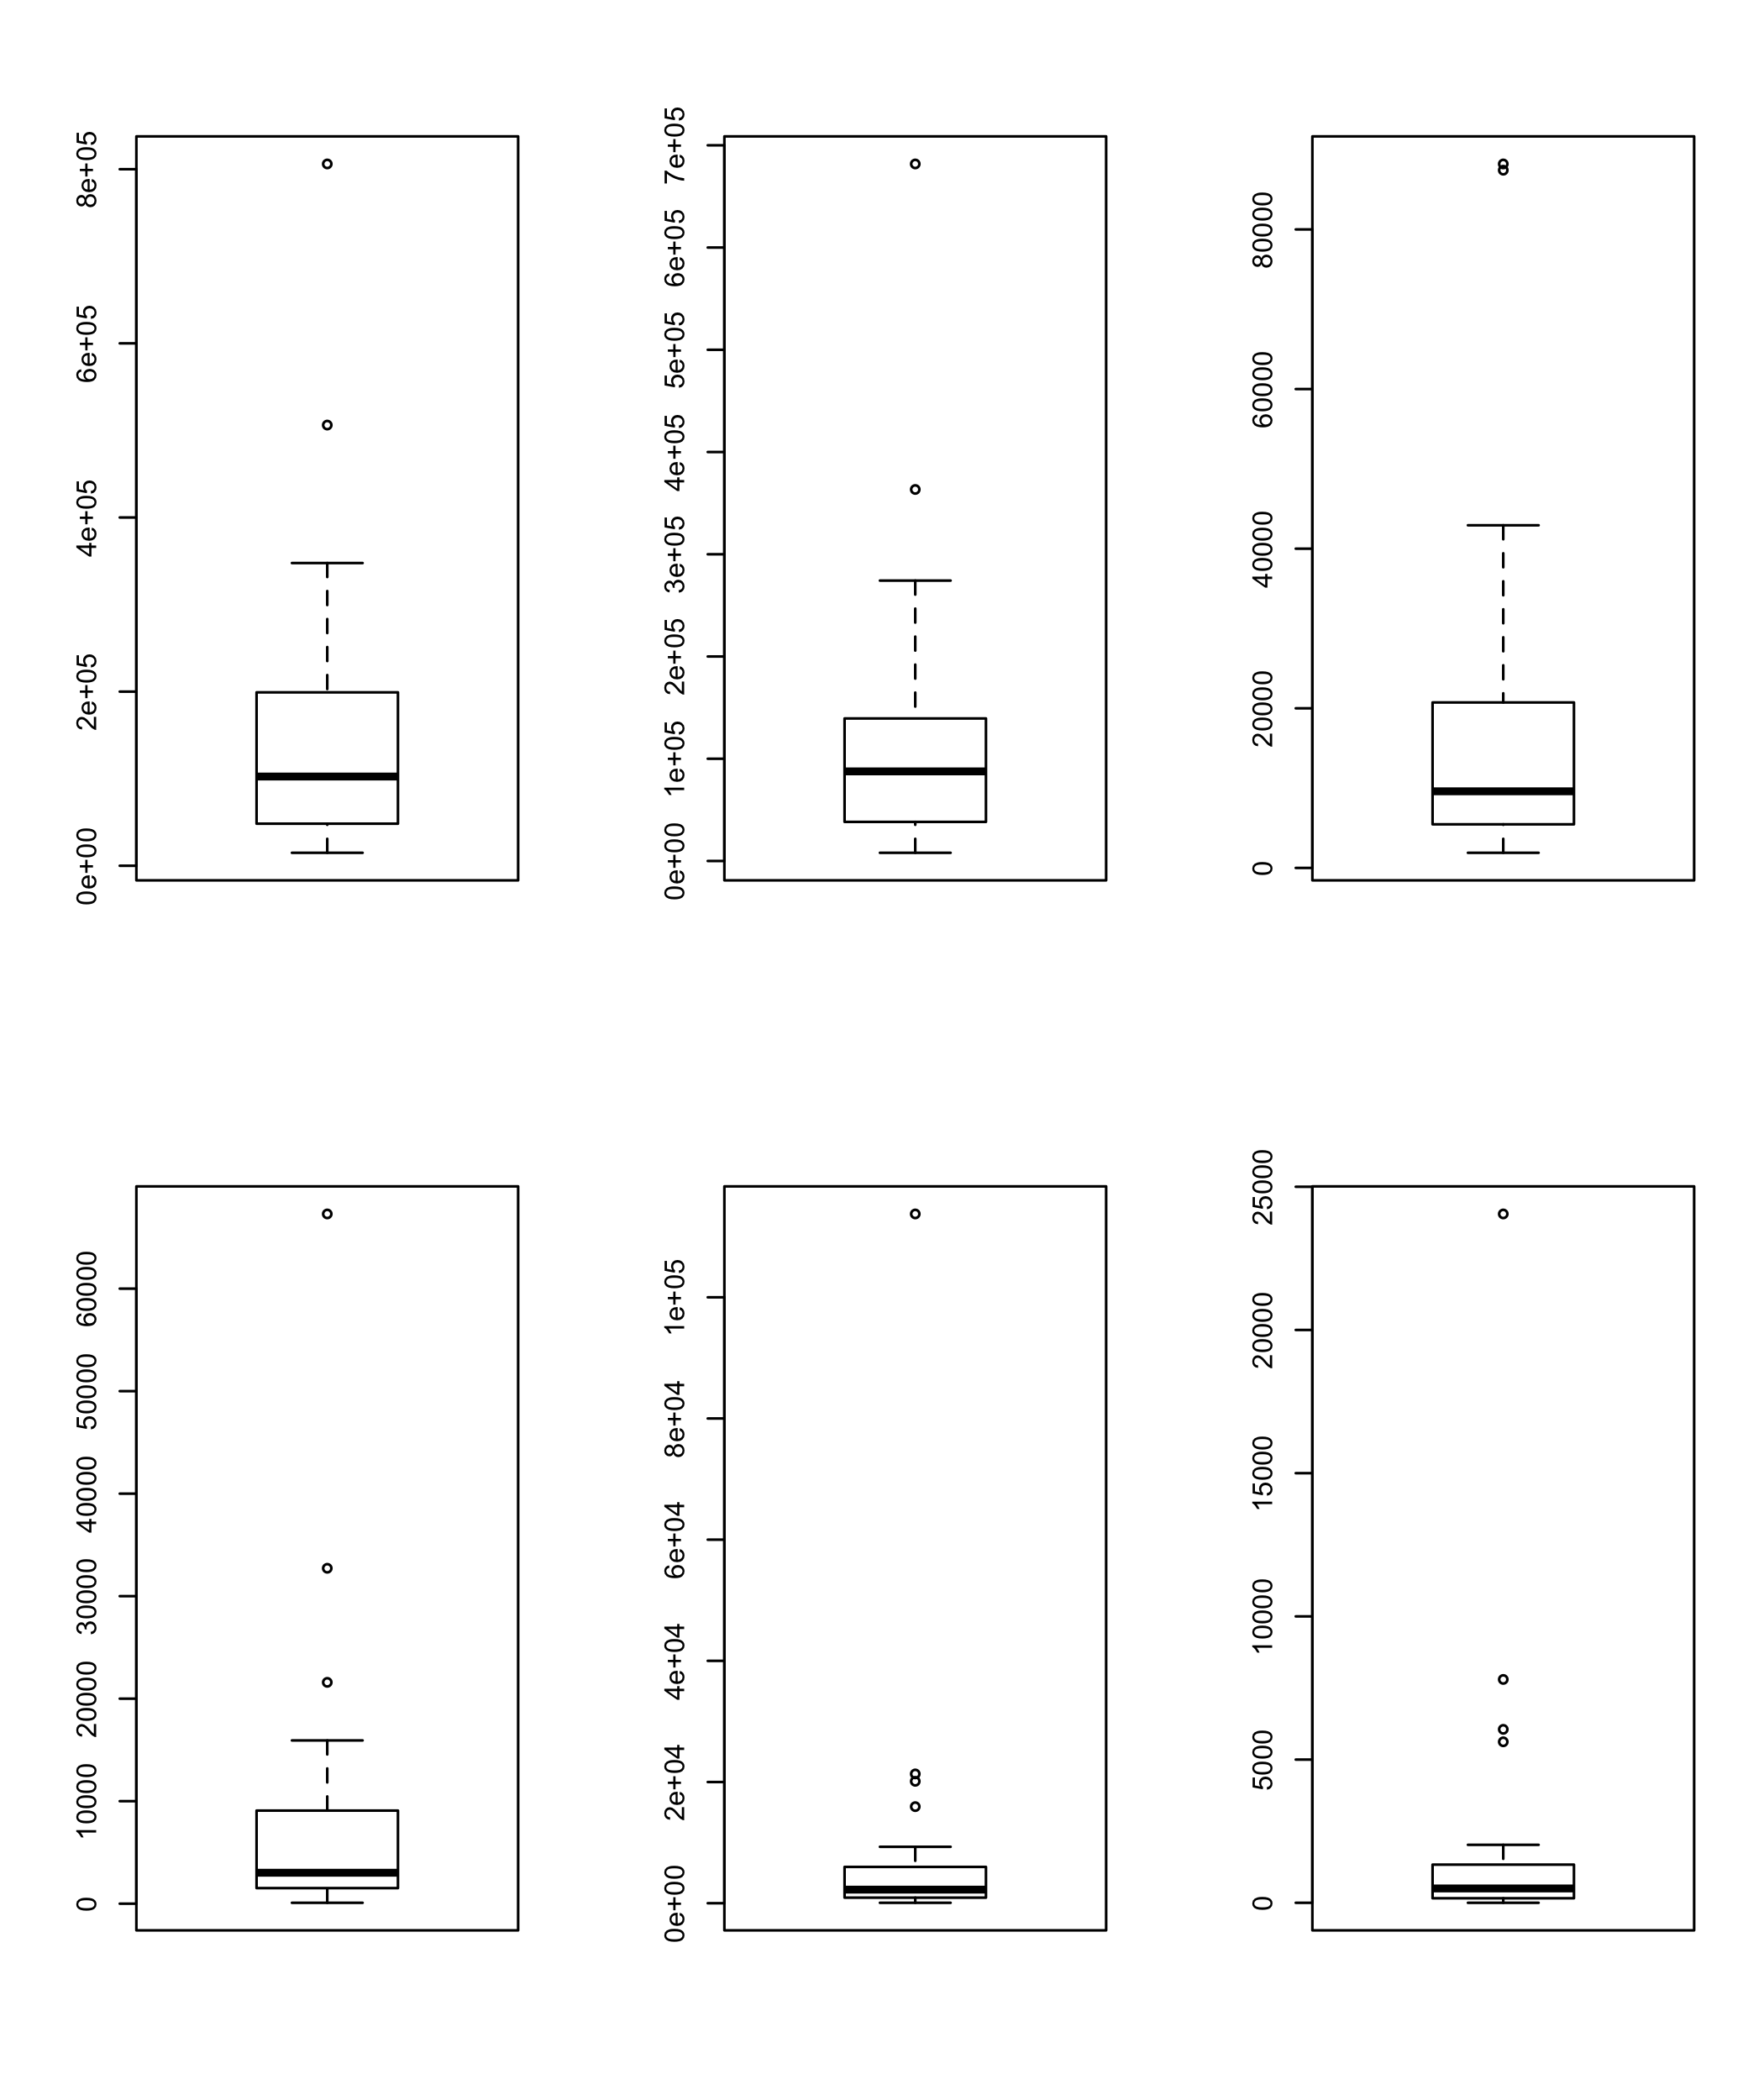
\includegraphics[width=\linewidth]{prueba1.png}
	\caption{Box plots of the variables but ordered individually.}\label{fig2}
\end{figure}

\clearpage

Now that we have a better view of the plots, we can appreciate that the outliers of the \textit{Public services} variable are bigger than \textit{Comercial, Industrial} and \textit{Pipe} variables. Knowing this and the big gap between domestic and all the other variables, we want to know which state is the one consuming the most water resources across all of the variables. \\

To be able to do this, we search in each variable the maximum value using the \textit{max} function, and we save it in another variable as a key number with the function \textit{which.max}, that will allow us to later search it in the variable \textit{States}, which holds a list of all the federative states. In Figure \ref{fig3} we see a bar graph that show the states that take most of the resources and cause those big outliers.\\

\begin{figure}[htp]
	\centering
	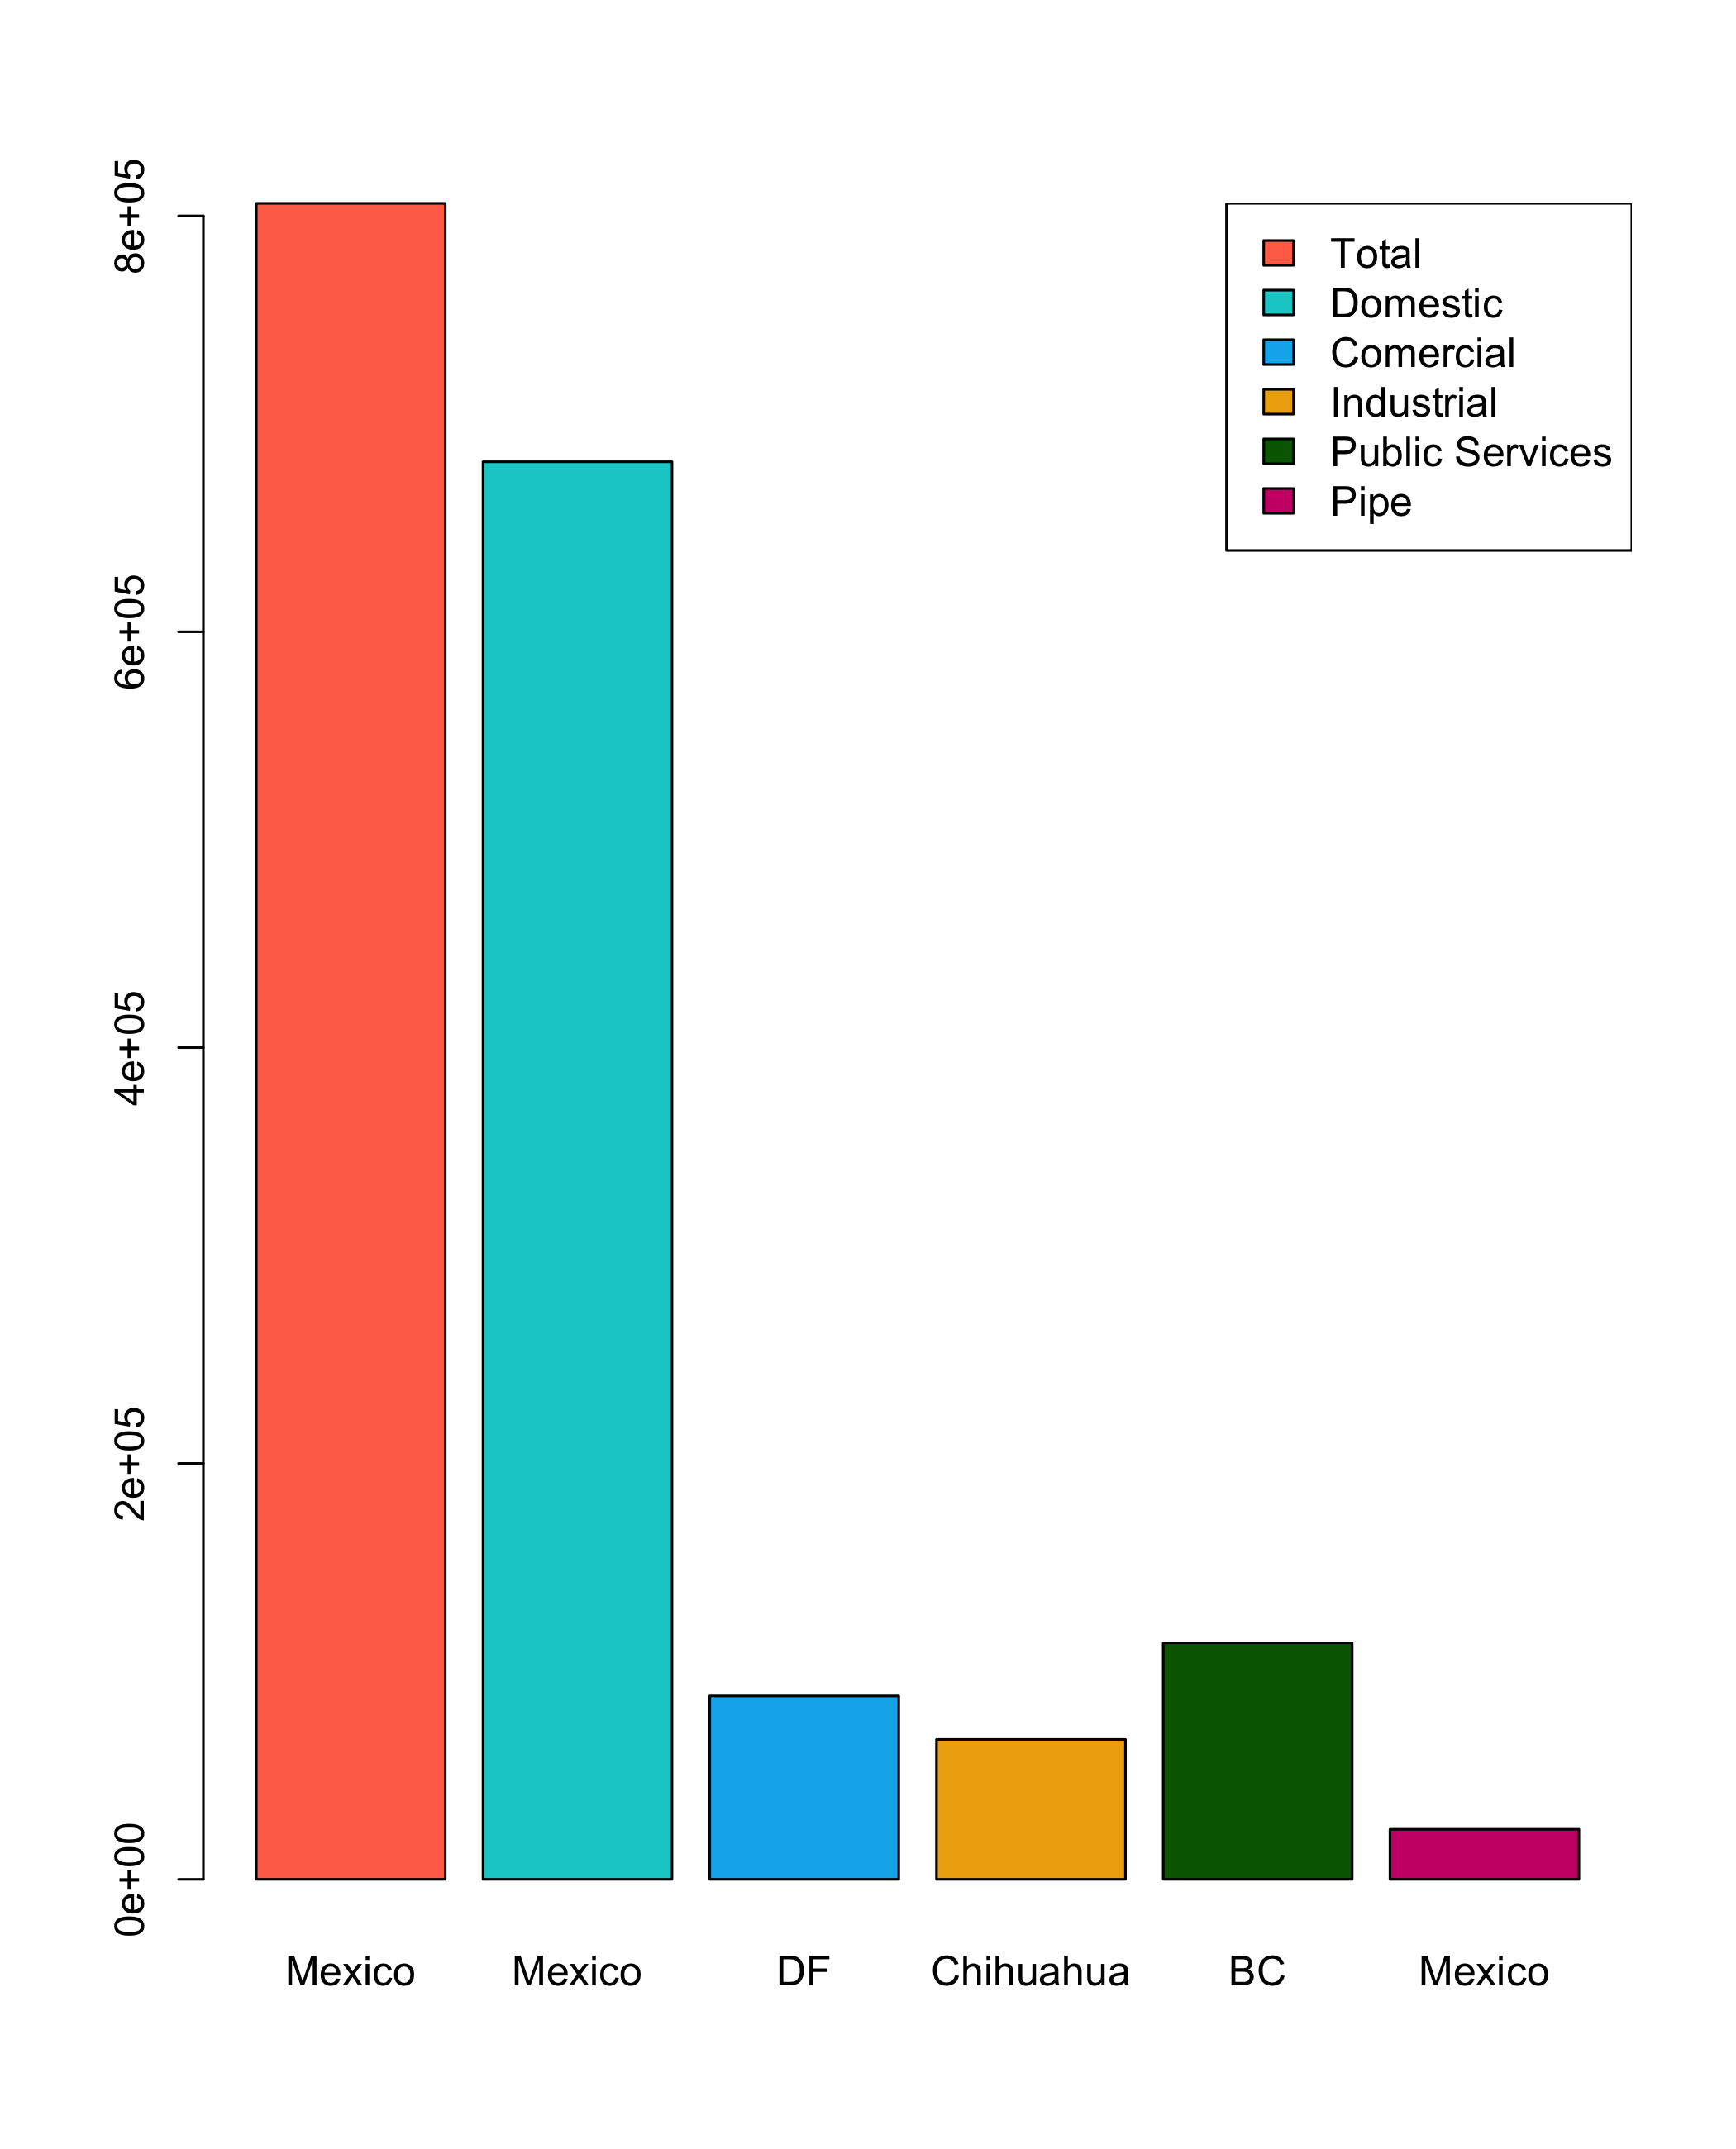
\includegraphics[width=\linewidth]{histo.png}
	\caption{Comparison of all the maximum values of each variable and to what state they correspond to.}\label{fig3}
\end{figure}

\clearpage
We confirm more visually that the outlier of the \textit{Public services} variable were in fact bigger than the other three.\\

Mexico city as the place that consumes more water generally and in \textit{Domestic} and \textit{Pipe} aspects comes to no surprise when we examine information outside the given dataset like the population of this state. In the density of population study made by the same organization, we find that the density in Mexico city is 724.2 inhabitants per square kilometer. The second most populated state is Morelos is of 390.2 inhabitants per square kilometer, which is almost half of the population of Mexico city\cite{ine2}.\\

In the industrial front, Chihuahua as well as other northern states are important points of the industry for Mexico, and in the case of Chihuahua, 95 percent of establishments are immersed in industrial businesses of the state\cite{industria}. As for the \textit{Public service}, they do not specify what areas this englobes, so we have shortage of information to make conclusions for this results.\\

In the Origin file, they only have two columns. The name of the federative state and the volume of water extracted from surface and subsoil mantles represented in thousands cubic meters. With this information, in Figure \ref{fig4} we put the income of water from all of the surface and subsoil mantles, and we compare it to the \textit{Total} variable, which represents all of the utilization of the water resources in Mexico.\\

\begin{figure}[htp]
	\centering
	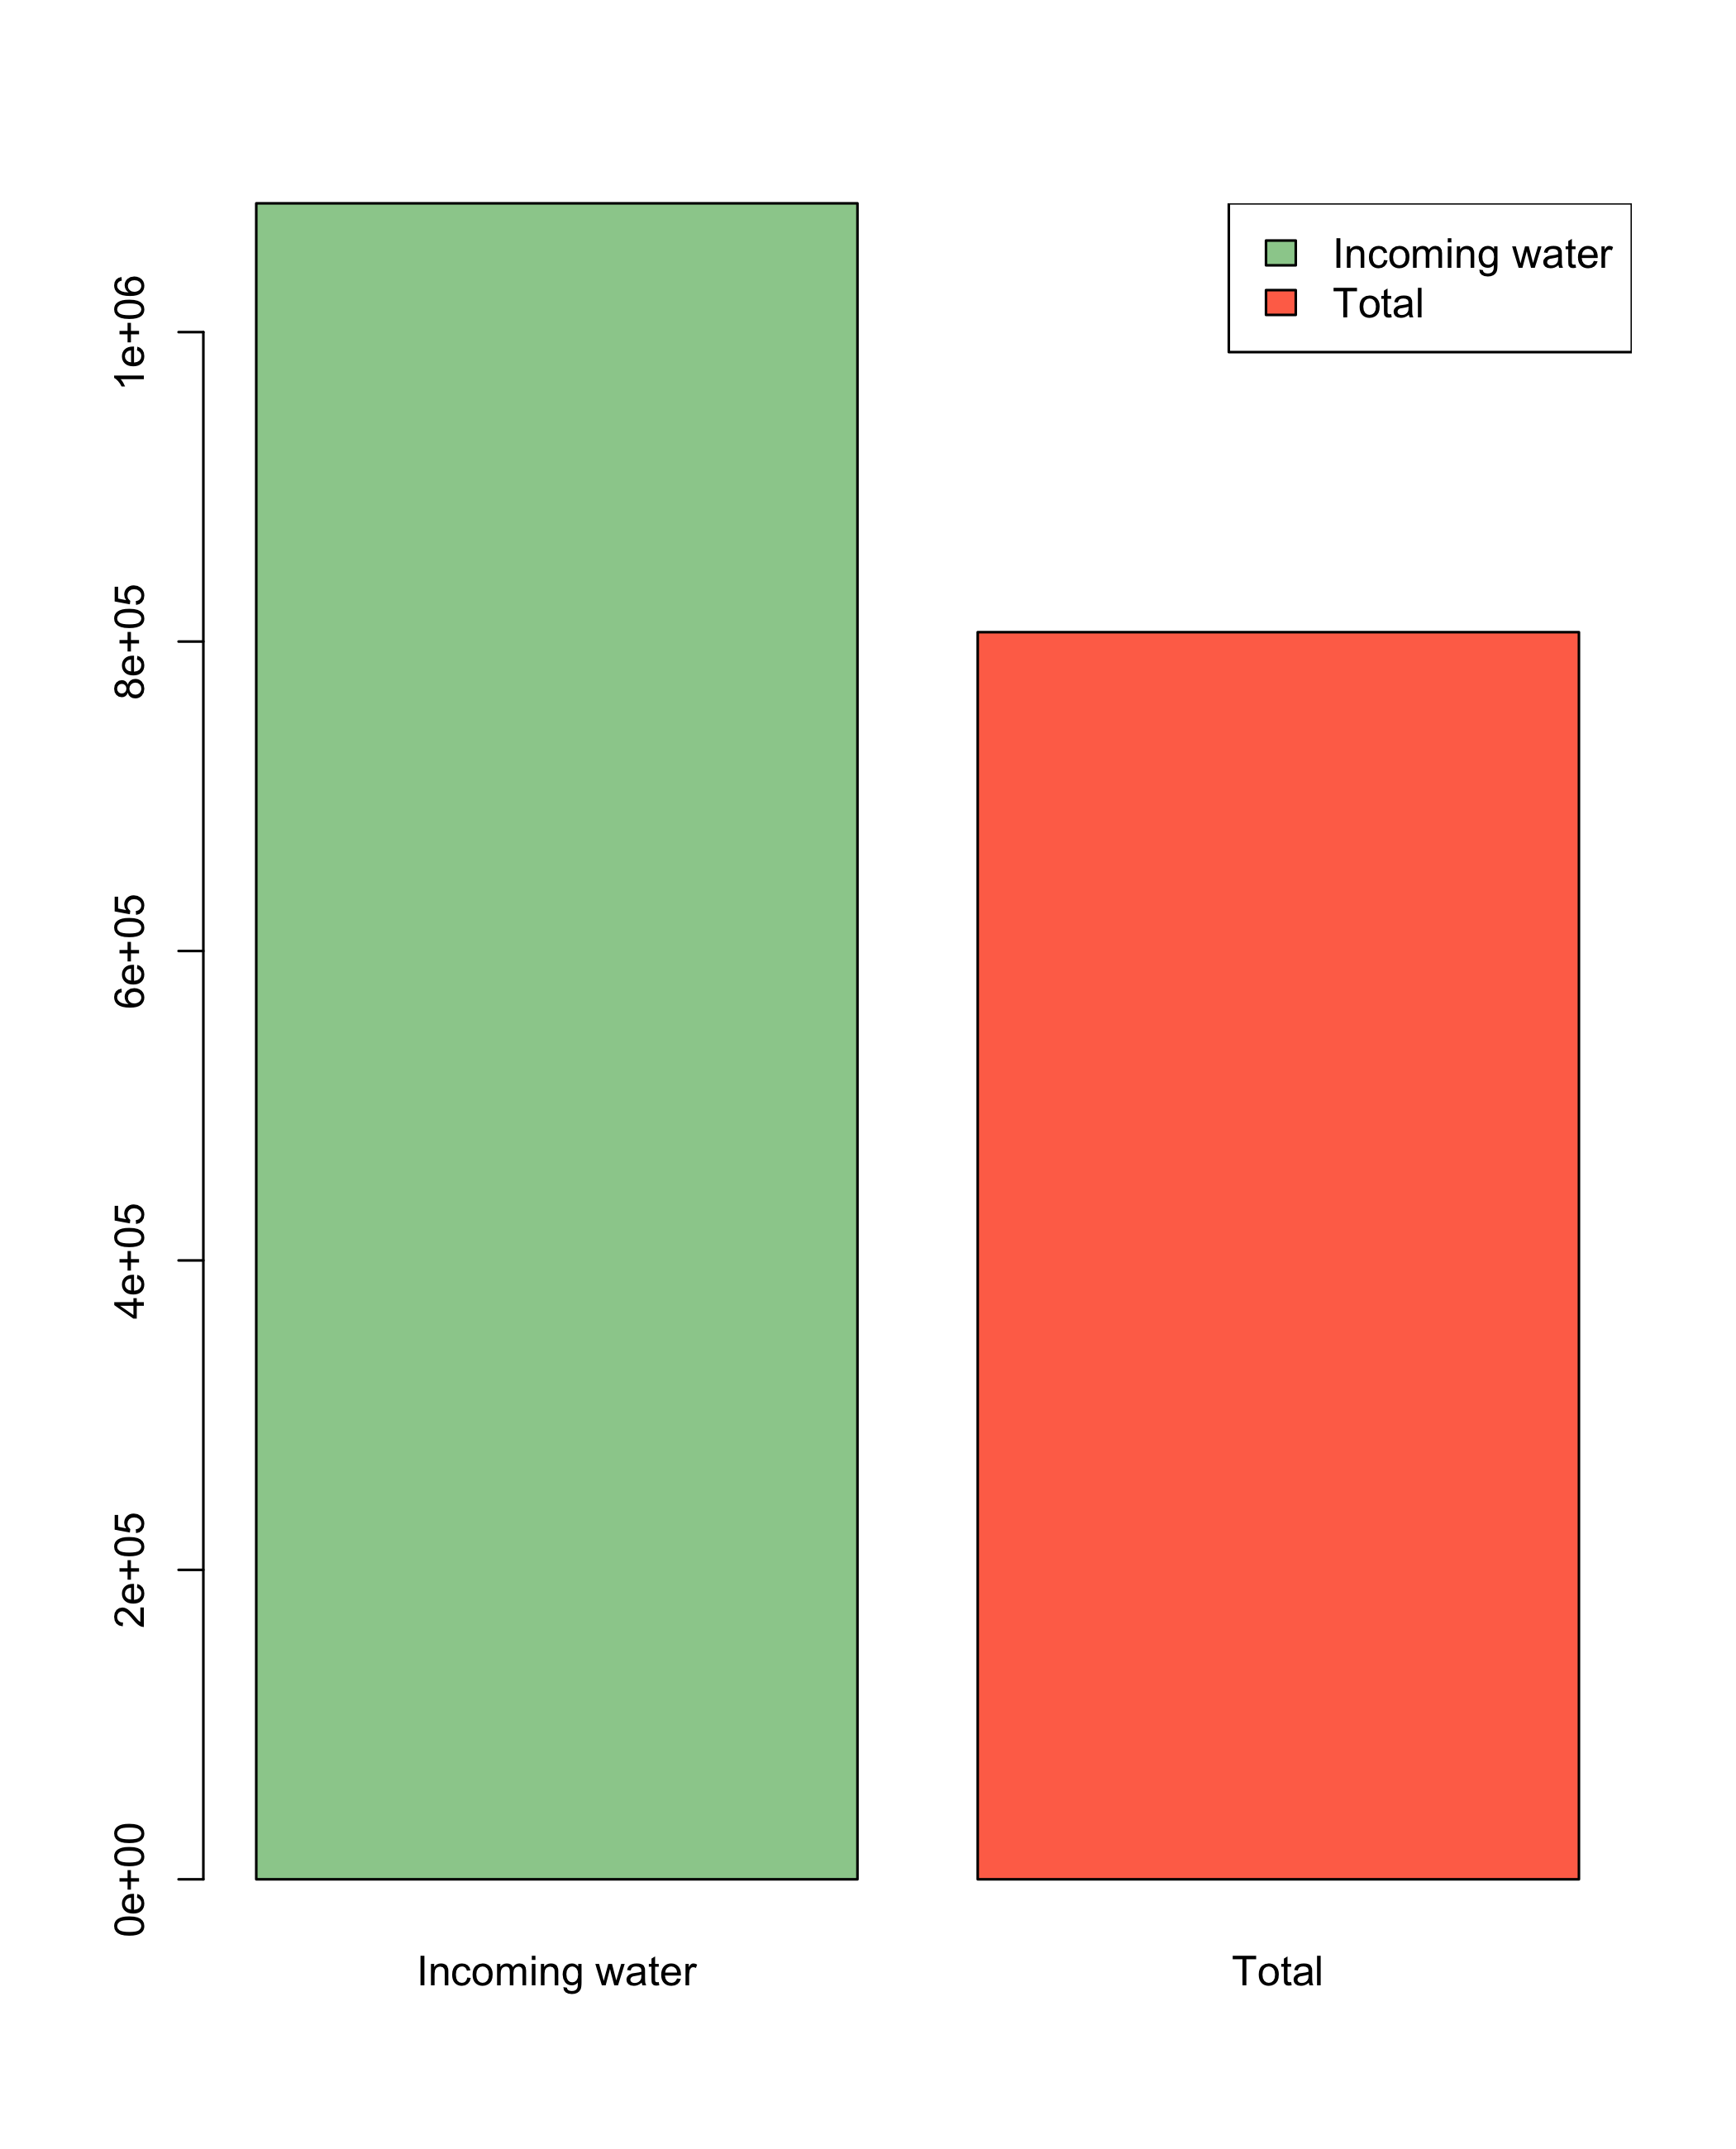
\includegraphics[width=\linewidth]{histo2.png}
	\caption{All the produced water in Mexico compared to the total of water used. }\label{fig4}
\end{figure}
\clearpage

As we can appreciate in Figure \ref{fig4} almost a quarter of the income water goes to exportation.\\

\section{Conclusions}

Choosing the subject of environment was a very quick decision, but now after reviewing the data and the plots made, I see another perspective to a problem faced in my hometown. Here in Tamaulipas, we make use of pipes of water and water tanks, because all year long, except on rainy season, we only have running water very early in the morning. This is, according to my parents, because the two only sources of water that we have are two dams that we share with Nuevo Leon and Texas. Seeing how much water goes to exportation and using it for industrial proposes, now I have a better clue as to why the shortage of water happens in my state.\\

\begin{thebibliography}{4}

\bibitem{ine1} INEGI - Quienes somos. \url{https://www.inegi.org.mx/inegi/contenido/instituto.html#:~:text=Somos\%20un\%20organismo\%20p\%C3\%BAblico\%20aut\%C3\%B3nomo,nuestro\%20pa\%C3\%ADs\%20y\%20ayudar\%20a} Accessed: 07/09/2020.

\bibitem{ine2} INEGI - Poblaci\'on. \url{https://www.inegi.org.mx/temas/estructura/default.html\#Tabulados}. Accessed:07/09/2020.

\bibitem{ine3} INEGI - Medio Ambiente. \url{https://www.inegi.org.mx/temas/agua/default.html#Tabulados}. Accessed:07/09/2020

\bibitem{industria} Industria y desarrollo enon\'omico y regional. \url{http://www.chihuahua.gob.mx/atach2/sf/uploads/indtfisc/Plan\%20Estatal\%20de\%20Desarrollo\%202004-2010/industria.pdf}. Accessed:07/09/2020

\end{thebibliography}
 
\end{document}